\section*{ÔN TẬP CHƯƠNG I}
\setcounter{ex}{0}\setcounter{bt}{0}
\Opensolutionfile{ans}[ans/ans-KTTX-1-1]
\TN
\begin{ex}%[0K1Y1-2]
Trong các mệnh đề sau mệnh đề nào đúng?
\choice
{ $\dfrac{3}{2}$ là số nguyên}
{ $2$ là số chính phương}
{\True $2$ là số nguyên tố}
{ $2023$ chia hết cho $3$}
\loigiai{
Số $2$ là số tự nhiên lớn hơn $1$ chỉ có một ước lớn hơn $1$ là chính nó nên $2$ là số nguyên tố.}
\end{ex}

\begin{ex}%[0K1Y1-3]
Cho mệnh đề $P:"\forall x\in \mathbb{R},x^2+x+1>0"$. Mệnh đề phủ định của mệnh đề $P$ là:
\choice
{ $"\forall x\in \mathbb{R},x^2+x+1<0"$}
{ $"\forall x\in \mathbb{R},x^2+x+1\le 0"$}
{\True $"\exists x\in \mathbb{R},x^2+x+1\le 0"$}
{ $"\exists x\in \mathbb{R},x^2+x+1>0"$}
\loigiai{
Phủ định của mệnh đề $"\forall x\in \mathbb{R},x^2+x+1>0"$ là mệnh đề $"\exists x\in \mathbb{R},x^2+x+1\le 0"$.}
\end{ex}

\begin{ex}%[0K1Y1-3]
Mệnh đề phủ định của mệnh đề "$2018$ là một số chẵn'' là
\choice
{$2018$ không là một số lẻ}
{$-2018$ không là một số chẵn}
{$-2018$ là một số lẻ}
{\True $2018$ không là một số chẵn}
\loigiai{
"$2018$ không là một số chẵn'' là mệnh đề phủ định của "$2018$ là một số chẵn''.
}
\end{ex}

\begin{ex}%[0K1Y2-1]%[0-GK1-NH22-23--TeamTeXHoa--Sơn Bùi]
Hình vẽ nào sau đây (phần không bị gạch) minh hoạ cho tập hợp $[1 ; 4]$?
\choice
{\begin{tikzpicture}[line join=round, line cap=round,>=stealth,thick]
\tikzset{label style/.style={font=\footnotesize}}
\fill[pattern=north east lines](4,-0.15)rectangle(5,0.15);
\fill[pattern=north east lines](0,-0.15)rectangle(1,0.15);
\draw[->] (0,0)--(5,0);
\draw (1,0) node {$\big($} (1,0) node[below=6pt]{$1$};
\draw (4,0) node {$\big]$} (4,0) node[below=6pt]{$4$};
\end{tikzpicture}}
{\begin{tikzpicture}[line join=round, line cap=round,>=stealth,thick]
\tikzset{label style/.style={font=\footnotesize}}
\fill[pattern=north east lines](4,-0.15)rectangle(5,0.15);
\fill[pattern=north east lines](0,-0.15)rectangle(1,0.15);
\draw[->] (0,0)--(5,0);
\draw (1,0) node {$\big[$} (1,0) node[below=6pt]{$1$};
\draw (4,0) node {$\big)$} (4,0) node[below=6pt]{$4$};
\end{tikzpicture}}
{\begin{tikzpicture}[line join=round, line cap=round,>=stealth,thick]
\tikzset{label style/.style={font=\footnotesize}}
\fill[pattern=north east lines](4,-0.15)rectangle(5,0.15);
\fill[pattern=north east lines](0,-0.15)rectangle(1,0.15);
\draw[->] (0,0)--(5,0);
\draw (1,0) node {$\big($} (1,0) node[below=6pt]{$1$};
\draw (4,0) node {$\big)$} (4,0) node[below=6pt]{$4$};
\end{tikzpicture}}
{\True \begin{tikzpicture}[line join=round, line cap=round,>=stealth,thick]
\tikzset{label style/.style={font=\footnotesize}}
\fill[pattern=north east lines](4,-0.15)rectangle(5,0.15);
\fill[pattern=north east lines](0,-0.15)rectangle(1,0.15);
\draw[->] (0,0)--(5,0);
\draw (1,0) node {$\big[$} (1,0) node[below=6pt]{$1$};
\draw (4,0) node {$\big]$} (4,0) node[below=6pt]{$4$};
\end{tikzpicture}}
\loigiai{}
\end{ex}

\begin{ex}%[0K1Y1-3]
Tìm mệnh đề phủ định của mệnh đề sau:  $ \exists x\in \mathbb{Q}\colon x^2-7\geq 0 $.
\choice
{$ \forall x\in \mathbb{Q}\colon x^2-7\leq 0 $}
{$ \exists x\in \mathbb{Q}\colon x^2-7< 0 $}
{$ \forall x\in \mathbb{Q}\colon x^2-7\geq 0 $}
{\True $ \forall x\in \mathbb{Q}\colon x^2-7<0 $}
\loigiai{
Ta có phủ định của mọi là tồn tại và phủ định của không âm là âm nên mệnh đề phủ định của mệnh đề đã cho là  $ \forall x\in \mathbb{Q}\colon x^2-7<0 $.
}
\end{ex}

\begin{ex}%[0K1Y1-3]
Phủ định của mệnh đề $"\exists x\in \mathbb{R},5x-3x^2=0"$ là mệnh đề
\choice
{ $"\exists x\in \mathbb{R},5x-3x^2\ne 0"$}
{ $"\forall x\in \mathbb{R},5x-3x^2=0"$}
{\True $"\forall x\in \mathbb{R},5x-3x^2\ne 0"$}
{ $"\exists x\in \mathbb{R},5x-3x^2\ge 0"$}
\loigiai{
Phủ định của mệnh đề $"\exists x\in \mathbb{R},5x-3x^2=0"$ là mệnh đề $"\forall x\in \mathbb{R},5x-3x^2\ne 0"$.}
\end{ex}

\begin{ex}%[0K1Y2-1]
Cho hai tập hợp $ A=\{1;5;9;13;17;21;25\} $  và $ B=\{0;1;3;5;10;13\} $. Tìm  $ A\cap B $.
\choice
{$ A\cap B =\{0;1;3;5;9;10;13;17;21;25\}$}
{\True $ A\cap B =\{1;5;13\}$}
{$ A\cap B =\{9;17;21;25\}$}
{$ A\cap B =\{0;3;10\}$}
\loigiai{
Ta có 	$ A\cap B =\{1;5;13\}$.
}
\end{ex}

\begin{ex}%[0-GK1-NH22-23--TeamTeXHoa--Don Lee]%[0K1Y1-2]
Tìm mệnh đề \textbf{đúng}?
\choice
{\lq\lq$\exists x\in\mathbb{R}\colon x^2+3=0$\rq\rq}
{\lq\lq$\forall x\in\mathbb{Z}\colon x^5>x^2$\rq\rq}
{\True \lq\lq$\forall x\in\mathbb{N}\colon (2x+1)^2-1\, \text{chia hết cho}\, 4$\rq\rq}
{\lq\lq$\exists x\in\mathbb{R}\colon x^4+3x^2+2=0$\rq\rq}
\loigiai{
Ta có $(2x+1)^2-1=(2x+1-1)(2x+1+1)=2x(2x+2)=4x(x+1)\vdots 4,\,\,\forall x\in\mathbb{N}$.\\
Suy ra \lq\lq$\forall x\in\mathbb{N}\colon (2x+1)^2-1\, \text{chia hết cho}\, 4$\rq\rq\, là mệnh đề đúng.
}
\end{ex}


\begin{ex}%[0K1Y1-3]
Mệnh đề phủ định của mệnh đề \lq\lq $\forall x\in \mathbb{R}, \ x^2+x+5>0$\rq\rq \ là
\choice
{\True \lq\lq$\exists x\in \mathbb{R},\ x^2+x+5\le 0$\rq\rq }
{\lq\lq$\forall x\in \mathbb{R},\ x^2 +x+5\le 0$\rq\rq}
{\lq\lq$\exists x\in \mathbb{R},\ x^2+x+5<0$\rq\rq	}
{\lq\lq$\forall x\in \mathbb{R},\ x^2+x+5<0$\rq\rq}

\loigiai{ Phủ định của mệnh đề \lq\lq $\forall x\in \mathbb{R}, \ x^2+x+5>0$\rq\rq \ là mệnh đề
\lq\lq$\exists x\in \mathbb{R},\ x^2+x+5\le 0$\rq\rq.
}
\end{ex}


\begin{ex} %[0K1Y2-1]
Cho hai tập hợp $X = \left\{ { - 1\,;\,2\,;\,4\,;\,7\,;\,9} \right\}$  và $Y = \left\{ { - 1\,;\,0\,;\,7\,;\,10} \right\}$  . Tập hợp $X \cap Y$  có bao
nhiêu phần tử?
\choice
{ $ 3 $ }
{ $ 7 $ }
{\True $ 2 $ }
{ $ 5 $ }
\loigiai{$ X\cap Y= \{-1;7\} $ có 2 phần tử.
}
\end{ex}

\begin{ex}%[0K1Y1-4]%[0K1Y1-4]%[0K1Y1-4]
Mệnh đề đảo của mệnh đề $P\Rightarrow Q$ là mệnh đề nào?
\choice
{\True $Q\Rightarrow P$}
{$Q\Rightarrow\overline{P}$}
{$Q\Rightarrow\overline{P}$}
{$\overline{Q}\Rightarrow P$}
\loigiai{
Mệnh đề đảo của mệnh đề $P\Rightarrow Q$ là mệnh đề $Q\Rightarrow P$.
}
\end{ex}

\begin{ex}%[0K1Y1-3]
Tìm mệnh đề phủ định của mệnh đề sau:  $ 7 $ là số nguyên tố.
\choice
{$ 7 $  có phải là số nguyên tố không?}
{$ 7 $  là số chính phương}
{\True $ 7 $  không phải là số nguyên tố}
{$ 7 $  là số nguyên tố}
\loigiai{
Mệnh đề phủ định của mệnh đề đã cho là:  $ 7 $ không phải là số nguyên tố.
}
\end{ex}

\begin{ex}%[0K1Y1-3]
Phủ định của mệnh đề \lq\lq Phương trình $ ax^2+bx+c=0\ \left( a\ne 0 \right)$ vô nghiệm \rq\rq  \ là
\choice
{\True \lq\lq Phương trình $ ax^2+bx+c=0\ \left( a\ne 0 \right)$ có nghiệm \rq\rq }
{\lq\lq Phương trình $ ax^2+bx+c=0\ \left( a\ne 0 \right)$ có 2 nghiệm phân biệt\rq\rq }
{\lq\lq Phương trình $ ax^2+bx+c=0\ \left( a\ne 0 \right)$ có nghiệm kép\rq\rq }
{\lq\lq Phương trình $ ax^2 +bx+c=0\ \left( a\ne 0 \right)$ không có nghiệm\rq\rq }
\loigiai{ Phủ định của mệnh đề \lq\lq Phương trình $ ax^2+bx+c=0\ \left( a\ne 0 \right)$ vô nghiệm \rq\rq  \ là mệnh đề \\ \lq\lq Phương trình $ ax^2+bx+c=0\ \left( a\ne 0 \right)$ có nghiệm \rq\rq.
}
\end{ex}


\begin{ex}%[0K1Y2-4]%[0-GK1-NH22-23--TeamTeXHoa--Sơn Bùi]
Cho hai tập hợp $A=\{1 ; 2 ; 3 ; 4 ; 5 ; 6 ; 7 ; 8 ; 9\}$; $B=\{0 ; 1 ; 2 ; 3 ; 4 ; 5\}$. Hiệu của hai tập hợp $A$ và $B$ là
\choice
{$A \setminus B=\{0 ; 1 ; 2 ; 3 ; 4 ; 5 ; 6 ; 7 ; 8 ; 9\}$}
{\True $A \setminus B=\{6 ; 7 ; 8 ; 9\}$ }
{$A \setminus B=\{1 ; 2 ; 3 ; 4 ; 5 ; 6 ; 7 ; 8 ; 9\}$ }
{$A \setminus B=\{1 ; 2 ; 3 ; 4 ; 5\}$}
\loigiai{$A \setminus B=\{6 ; 7 ; 8 ; 9\}$.}
\end{ex}

\begin{ex} %[0K1Y1-2]
Trong các mệnh đề sau, mệnh đề nào là mệnh đề \textbf{sai}?
\choice
{\True $ - \pi  <  - 2 \Leftrightarrow {\pi ^2} < 4$ }
{ $\pi  < 4 \Leftrightarrow {\pi ^2} < 16$ }
{ $\sqrt {23}  < 5 \Leftrightarrow 2\sqrt {23}  < 2\cdot 5$ }
{ $\sqrt {23}  < 5 \Leftrightarrow  - 2\sqrt {23}  >  - 2\cdot 5$ }
\loigiai{Mệnh đề "$ P\Rightarrow Q $" đúng khi và chỉ khi $ P,Q $ cùng đúng hoặc cùng sai.\\
Mệnh đề  \lq\lq$ - \pi  <  - 2 \Leftrightarrow {\pi ^2} < 4$ \rq\rq  là một mệnh đề đúng. Vì
\lq\lq $ - \pi  <  - 2 $\rq\rq   và   \lq\lq $ {\pi ^2} < 4$ \rq\rq  cùng đúng.
}
\end{ex}

\begin{ex}%[0K1Y2-2]
Cho tập hợp $A=\big\{1;2;3\big\}$. Tập hợp nào sau đây \textbf{không} là tập con của tập $A$?
\choice
{$\big\{1;2;3\big\}$}
{$\big\{1;2\big\}$}
{$\varnothing$}
{\True $\big\{1;3;4\big\}$}
\loigiai{
Tập hợp $\big\{1;3;4\big\}$ \textbf{không} là tập con của tập hợp $A$ vì có $4 \notin A$.
}
\end{ex}

\begin{ex}%[0K1B1-2]
Trong các mệnh đề sau, mệnh đề nào sai?
\choice
{Tam giác $ABC$ cân và có một góc bằng $60{}^\circ $ tương đương tam giác $ABC$ đều}
{Tam giác $ABC$ có ba góc bằng $60{}^\circ $ khi và chỉ khi tam giác $ABC$ đều}
{Tam giác $ABC$ có ba cạnh bằng nhau nếu và chỉ nếu tam giác $ABC$ đều}
{\True Tam giác $ABC$ cân là điều kiện cần và đủ để tam giác $ABC$ đều}
\loigiai{
“Nếu tam giác $ABC$ cân thì tam giác $ABC$ đều” là mệnh đề sai. Vậy mệnh đề ở phương án D là mệnh đề sai.}
\end{ex}

\begin{ex}%[0K1B1-4]%[0-GK1-NH22-23--TeamTeXHoa--Sơn Bùi]
Cách phát biếu nào sau đây \textbf{KHÔNG} dùng để phát biểu định lí toán học dạng $A \Rightarrow B$?
\choice
{Nếu $A$ thì $B$}
{$A$ kéo theo $B$}
{\True $A$ là điều kiện cần đề có $B$}
{$A$ là điều kiện đủ để có $B$}
\loigiai{}
\end{ex}

\begin{ex}%[0K1B2-3]
Cho hai tập hợp $A=\left\{ 1; 3; 5; 7; 9 \right\}$, $B=\left\{ 0; 1; 2; 4; 5; 6; 8 \right\}$. Tìm tập hợp $C=A\cup B$.
\choice
{ $C=\left\{ 3; 7; 9 \right\}$}
{ $C=\left\{ 1; 5 \right\}$}
{ $C=\left\{ 1; 3; 5; 7; 9 \right\}$}
{\True $C=\left\{ 0; 1; 2; 3; 4; 5; 6; 7; 8; 9 \right\}$}
\loigiai{
Ta có $C=\left\{ 0; 1; 2; 3; 4; 5; 6; 7; 8; 9 \right\}$.}
\end{ex}

\begin{ex}%[0K1B2-1]
Liệt kê các phần tử của tập hợp $A=\left\{ x \in \mathbb{Z} \mid 2x^2+3x+1=0\right\}$.
\choice
{$A=\left\{ -1;-\dfrac{1}{2} \right\}$}
{\True $A=\big\{-1\big\}$}
{$A=\left\{ -\dfrac{1}{2} \right\}$}
{$A=\varnothing$}
\loigiai{
Ta có $2x^2+3x+1=0 \Leftrightarrow \hoac{&x=-\dfrac{1}{2} \notin \mathbb{Z}\\&x=-1 \in \mathbb{Z}.}$\\
Do đó $A=\big\{-1\big\}$.
}
\end{ex}

\begin{ex}%[0K1B2-1]%[0-GK1-NH22-23--TeamTeXHoa--Sơn Bùi]
Trong các tập hợp sau, tập nào khác rỗng?
\choice
{$C=\left\{x \in \mathbb{R}\,\middle|\,\dfrac{x}{x^{2}+1}=1\right\}$}
{$A=\left\{x \in \mathbb{R} \,\middle|\, x^{2}-2 x+3=0\right\}$ }
{\True $D=\left\{x \in \mathbb{Q} \,\middle|\, x^{3}+8=0\right\}$}
{$B=\left\{x \in \mathbb{Q} \,\middle|\, 2 x^{2}-1=0\right\}$}
\loigiai{\begin{itemize}
\item $C=\left\{x \in \mathbb{R} \,\middle|\, \dfrac{x}{x^{2}+1}=1\right\}=\left\{x \in \mathbb{R} \,\middle|\, x^{2}-x+1=0\right\}=\varnothing$.
\item $A=\left\{x \in \mathbb{R} \,\middle|\, x^{2}-2 x+3=0\right\}=\varnothing$.
\item $B=\left\{x \in \mathbb{Q} \,\middle|\, 2 x^{2}-1=0\right\}=\left\{x \in \mathbb{Q} \,\middle|\, x=\dfrac{\pm \sqrt{2}}{2}\right\}=\varnothing$.
\item $D=\left\lbrace x \in \mathbb{Q} \,\middle|\, x^{3}+8=0\right\rbrace =\left\lbrace x \in \mathbb{Q} \,\middle|\, x=-2\right\rbrace=\{-2\} \neq \varnothing$.
\end{itemize}
}
\end{ex}

\begin{ex}%[0K1B1-4]
Mệnh đề nào sau đây đúng?
\choice
{Hai tam giác bằng nhau là điều kiện cần để diện tích của chúng bằng nhau}
{Số tự nhiên chia hết cho $ 5 $ là điều kiện đủ để nó có tận cùng bằng $ 5  $}
{Điều kiện đủ để hình bình hành $A B C D$ là hình thoi}
{\True Tứ giác $A B C D$ là hình thoi là điều kiện cần và đủ để tứ giác đó là hình bình hành và có hai đường chéo vuông góc với nhau}
\loigiai{
\begin{itemize}
\item 	Mệnh đề \lq\lq Hai tam giác bằng nhau là điều kiện cần để diện tích của chúng bằng nhau\rq\rq~sai vì  giả sử có hai tam giác diện tích đều bằng 6 nhưng một hình có chiều cao là $ 3 $, đáy là $ 4  $. Một hình có chiều cao là $ 2  $, đáy là $ 6  $. Hai tam giác đó không bằng nhau.
\item Mệnh đề \lq\lq Số tự nhiên chia hết cho $ 5 $ là điều kiện đủ để nó có tận cùng bằng $ 5  $\rq\rq~ sai vì số tự nhiên chia hết cho $ 5 $ thì nó có tận cùng là $ 0 $ hoặc $ 5  $.
\item  Mệnh đề \lq\lq Điều kiện đủ để hình bình hành $A B C D$ là hình thoi\rq\rq~ sai vì  thiếu một vế.
\end{itemize}
}
\end{ex}

\begin{ex}%[0K1B1-4]
Xét mệnh đề $P$: \lq\lq Tam giác $A B C$ vuông tại $A$\rq\rq ~và mệnh đề $Q$: \lq\lq Tam giác $A B C$ có $B C^2=A B^2+A C^2$\rq\rq. Phát biểu nào sau đây là mệnh đề $P \Rightarrow Q$ ?
\choice
{$B C^2=A B^2+A C^2$ là điều kiện cần và đủ để tam giác $A B C$ vuông tại $A$}
{Tam giác $A B C$ vuông tại $A$ khi và chỉ khi $B C^2=A B^2+A C^2$}
{\True Nếu tam giác $A B C$ vuông tại $A$ thì $B C^2=A B^2+A C^2$}
{Nếu tam giác $A B C$ có $B C^2=A B^2+A C^2$ thì tam giác đó vuông tại $A$}
\loigiai{
Nếu tam giác $A B C$ vuông tại $A$ thì $B C^2=A B^2+A C^2$.
}
\end{ex}

\begin{ex}%[0K1B2-1]
Tập hợp nào sau đây là tập hợp rỗng?
\choice
{ $\left\{ x\in \mathbb{Z}: 6x^2-7x+1=0 \right\}$}
{ $\left\{ x\in \mathbb{Z}: | x |<1  \right\}$}
{ \True $\left\{ x\in \mathbb{Q}: x^2-4x+2=0  \right\}$}
{ $\left\{ x\in \mathbb{R}\big| x^2-4x+3=0  \right\}$}
\loigiai{

Ta có $x^2-4x+2=0\Leftrightarrow \hoac{
& x=2+\sqrt{2}\notin \mathbb{Q} \\
& x=2-\sqrt{2}\notin \mathbb{Q}.
}$\\
Vậy $\left\{ x\in \mathbb{Q}: x^2-4x+2=0  \right\}=\varnothing$. }
\end{ex}

\begin{ex}%[0-GK1-NH22-23--TeamTeXHoa--Đào Trung Kiên]%[0K1B1-5]
Kí hiệu $A$ là tập hợp các cầu thủ $x$ trong đội tuyển bóng đá, $P(x)$ là mệnh đề chứa biến \lq\lq$x$ cao trên $170$ cm\rq\rq. Mệnh đề: \lq\lq$\forall x\in A, P(x)$\rq\rq\quad khẳng định rằng
\choice
{\True Mọi cầu thủ trong đội tuyển bóng đá đều cao trên $170$ cm}
{Có một cầu thủ trong đội tuyển bóng đá cao trên $170$ cm}
{Bất cứ ai cao trên $170\mathrm{~cm}$ đều là cầu thủ của đội tuyển bóng đá}
{Có một số người cao trên $170\mathrm{~cm}$ là cầu thủ của đội tuyển bóng đá}
\loigiai{Mệnh đề: \lq\lq$\forall x\in A, P(x)$\rq\rq\, có nghĩa là \lq\lq Mọi cầu thủ trong đội tuyển bóng đá đều cao trên $170$ cm\rq\rq.}
\end{ex}

\begin{ex}%[0K1B1-2]
Mệnh đề chứa biến  $P:\forall x \in \mathbb{R},\,\,{x^2} - 2 + a > 0$ với $ a $ là một số thực cho trước. Tìm tất cả các số thực $ a $  để  $ P $ đúng.
\choice
{ $a \le 2$ }
{$a < 2$  }
{ $a = 2$ }
{\True $a > 2$ }
\loigiai{
Điều kiện $ -2+a>0\Leftrightarrow a>2. $
}
\end{ex}

\begin{ex}%[0K1B1-5]
Viết mệnh đề sau bằng kí hiệu $\forall$ hoặc $\exists$: "Có một số nguyên bằng bình phương của chính nó''.
\choice
{$\exists x \in \mathbb{R},\,x^2-x=0$}
{$\exists x \in \mathbb{R},\,x=x^2$}
{$\forall x \in \mathbb{Z},\,x^2=x$}
{\True $\exists x \in \mathbb{Z},\,x=x^2$}
\loigiai{
$\exists x \in \mathbb{Z},\,x=x^2$: có một số nguyên bằng bình phương của chính nó.
}
\end{ex}

\begin{ex}%[0K1B2-1]
Một lớp có $ 45 $ học sinh. Mỗi em đều đăng ký chơi ít nhất một trong hai môn: bóng đá và bóng chuyền. Có $ 35 $ em đăng ký môn bóng đá, $ 15 $ em đăng ký môn bóng chuyền. Hỏi có bao nhiêu em đăng ký chơi cả $ 2 $ môn?
\choice
{ $ 30 $ }
{ $ 25 $ }
{\True $ 5 $ }
{ $ 10 $ }
\loigiai{Gọi $ A $ là tập các học sinh đăng ký chơi bóng đá; $ B $ là tập các học sinh đăng ký chơi bóng chuyền. Khi đó, $ A\cap B $ là tập các học sinh đăng ký cả hai môn và $ A\cup B $ là tập các học sinh đăng ký ít nhất một môn.
Ta có,
\[ n_{A\cap B}=n_{A}+n_{B}-n_{A\cup B}=35+15-45=5.
\]
}
\end{ex}

\begin{ex}%[0-GK1-NH22-23--TeamTeXHoa--Don Lee]%[0K1B2-3]
Cho các tập hợp $A=\{1;\,2;\,3;\,4\}$, $B=\{2;\,4;\,6;\,8\}$ và $C=\{3;\,4;\,5;\,6\}$. Chọn khẳng định \textbf{đúng}
\choice
{$A\cap B\cap C=\{1;\,2\}$}
{\True $A\cup(B\cap C)=\{1;2;\,3;\,4;\,6\}$}
{$(A\cup C)\cap B=\{1;\,2;\,4\}$}
{$(A\cup B)\cap C=\{2;\,4;\,6\}$}
\loigiai{
Ta có $B\cap C=\{4;\,6\}$ suy ra $A\cup(B\cap C)=\{1;2;\,3;\,4;\,6\}$.
}
\end{ex}

\begin{ex}%[0K1B1-2]
Trong các mệnh đề sau, mệnh đề nào có mệnh đề đảo {\bf{sai}}?
\choice
{Nếu tứ giác $ ABCD $  là hình bình hành thì tứ giác đó có một cặp cạnh đối song song và có độ dài bằng nhau}
{Nếu tam giác $ ABC $  đều thì tam giác đó có hai góc có số đo bằng $ 60^\circ $ }
{\True Nếu hai tam giác bằng nhau thì hai tam giác đó có diện tích bằng nhau}
{Nếu tứ giác $ ABCD $  có bốn góc vuông thì tứ giác đó là hình chữ nhật}
\loigiai{
Mệnh đề \lq\lq Nếu hai tam giác bằng nhau thì hai tam giác đó có diện tích bằng nhau\rq\rq\, có mệnh đề đảo là \lq\lq Nếu hai tam giác có diện tích bằng nhau thì hai tam giác đó bằng nhau\rq\rq.\\
Mệnh đề đảo này sai. Vì chẳng hạn, xét hai tam giác vuông có hai cạnh góc vuông lần lượt là $ 3 $, $ 4 $  và  $ 6 $, $ 2 $. Khi đó hai tam giác này có diện tích bằng nhau nhưng chúng không phải là hai tam giác bằng nhau.

}
\end{ex}
\TL
\begin{bt}%[0D1B4-2]
	Cho hai tập hợp $\mathrm{A}=[-2; 3]$ và $\mathrm{B}=(1;+\infty)$. Xác định các tập hợp sau và biểu diễn chúng lên trục số.
	$$
	\mathrm{A} \cap \mathrm{B};\, \mathrm{B} \setminus \mathrm{A}\, \text {và}\, \mathrm{C}_{\mathbb{R}} \mathrm{B}.
	$$
	\loigiai{\begin{multicols}{3}
			\begin{enumerate}[$\bullet$]
				\item $\mathrm{A} \cap \mathrm{B}=(1;3]$;
				\item $\mathrm{B} \setminus \mathrm{A}=(3;+\infty)$;
				\item $\mathrm{C}_{\mathbb{R}} \mathrm{B}=(-\infty;1]$.		
			\end{enumerate}
		\end{multicols}
		}
\end{bt}
\begin{bt}%[0D1B4-2]
	Xác định các tập hợp sau và biểu diễn chúng trên trục số.
	\begin{multicols}{3}
	\begin{enumerate}
		\item $(-\infty; 1) \cap(0;+\infty)$;
		\item $(4; 7] \cup(-1; 5)$;
		\item $(4; 7] \setminus(-3; 5]$		
	\end{enumerate}
	\end{multicols}
	
	\loigiai{
		\begin{enumerate}
			\item $(-\infty; 1) \cap(0;+\infty)=(0;1)$ được biểu diễn trên trục số là
			\begin{center}
				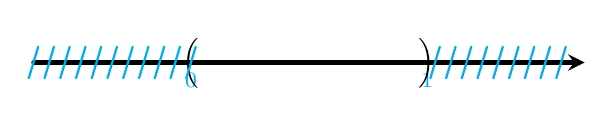
\begin{tikzpicture}[scale=1,>=stealth, font=\footnotesize, line join=round, line cap=round]
					\draw[->,ultra thick](0,0)--(7,0);
					\path 
					(2,0)coordinate (A)node[below=.2] {\color{cyan}$0$}node{$\Big($}
					(5,0)coordinate (B)node[below=.2] {\color{cyan}$1$}node{$\Big)$}
					;
					\foreach \i in {0,0.2,...,2}{
						\draw[color=cyan,thick](\i+.06,.2)--(\i-.06,-.2);
					}
					\foreach \i in {5.1,5.3,...,6.7}{
						\draw[color=cyan,thick](\i+.06,.2)--(\i-.06,-.2);
					}
				\end{tikzpicture}	
			\end{center}
			\item $(4; 7] \cup(-1; 5)=(-1;7]$ được biểu diễn trên trục số là
			\begin{center}
				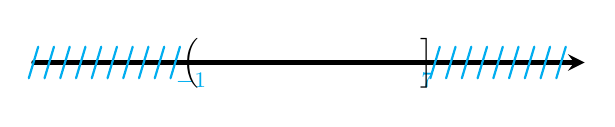
\begin{tikzpicture}[scale=1,>=stealth, font=\footnotesize, line join=round, line cap=round]
					\draw[->,ultra thick](0,0)--(7,0);
					\path 
					(2,0)coordinate (A)node[below=.2] {\color{cyan}$-1$}node{$\Big($}
					(5,0)coordinate (B)node[below=.2] {\color{cyan}$7$}node{$\Big]$}
					;
					\foreach \i in {0,0.2,...,1.8}{
						\draw[color=cyan,thick](\i+.06,.2)--(\i-.06,-.2);
					}
					\foreach \i in {5.1,5.3,...,6.7}{
						\draw[color=cyan,thick](\i+.06,.2)--(\i-.06,-.2);
					}
				\end{tikzpicture}	
			\end{center}
			\item $(4; 7] \setminus(-3; 5]=(5;7]$ được biểu diễn trên trục số là
			\begin{center}
				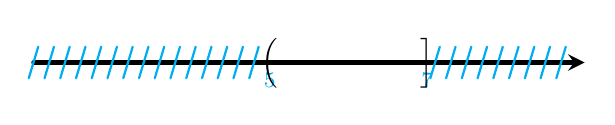
\begin{tikzpicture}[scale=1,>=stealth, font=\footnotesize, line join=round, line cap=round]
					\draw[->,ultra thick](0,0)--(7,0);
					\path 
					(3,0)coordinate (A)node[below=.2] {\color{cyan}$5$}node{$\Big($}
					(5,0)coordinate (B)node[below=.2] {\color{cyan}$7$}node{$\Big]$}
					;
					\foreach \i in {0,0.2,...,2.8}{
						\draw[color=cyan,thick](\i+.06,.2)--(\i-.06,-.2);
					}
					\foreach \i in {5.1,5.3,...,6.7}{
						\draw[color=cyan,thick](\i+.06,.2)--(\i-.06,-.2);
					}
				\end{tikzpicture}	
			\end{center}
		\end{enumerate}
	}
\end{bt}
% \begin{ex}%[0K1B2-2]
% Cho tập hợp $A=\left\{ -1;\,0;\,1;\,2;\,3 \right\}$. Số tập con gồm 2 phần tử của tập $A$ là
% \choice
% { $20$}
% {\True 10}
% { $12$}
% { $15$}
% \loigiai{
% Các tập con gồm 2 phần tử của tập hợp $A$ là: $\left\{ -1;\,0 \right\}$, $\left\{ -1;\,1 \right\}$, $\left\{ -1;2 \right\}$, $\left\{ -1;3 \right\}$, $\left\{ 0;1 \right\}$, $\left\{ 0;2 \right\}$, $\left\{ 0;\,3 \right\}$, $\left\{ 1;\,2 \right\}$, $\left\{ 1;\,3 \right\}$, $\left\{ 2;\,3 \right\}$.\\
% Vậy có 10 tập con gồm 2 phần tử của tập $A$.}
% \end{ex}

% \begin{ex}%[0K1K2-6]
% Cho khoảng $A=\left( 1;m+7 \right)$ và nửa khoảng $B=\left[ 2m+3;13 \right)$ ($m$ là tham số). Gọi $S$ là tập hợp tất cả các số nguyên $m$ sao cho $A\cup B=\left( 1;13 \right)$. Tổng các phần tử của tập hợp $S$ là
% \choice
% {\True $10$}
% { $9$}
% { $-5$}
% { $21$}
% \loigiai{
% Điều kiện đối với $m$ để tồn tại khoảng $A$ và nửa khoảng $B$ là \[\left\{ \begin{aligned}
% & m+7>1 \\
% & 2m+3<13 \\
% \end{aligned} \right.\Leftrightarrow -6<m<5. \left( * \right)\]
% Khi đó
% \[A\cup B=\left( 1\,;\,13 \right)\Leftrightarrow \left\{ \begin{aligned}
% & 2m+3>1 \\
% & 2m+3\le m+7 \\
% & m+7\le 13 \\
% \end{aligned} \right.\Leftrightarrow \left\{ \begin{aligned}
% & m>-1 \\
% & m\le 4 \\
% & m\le 6 \\
% \end{aligned} \right.\Leftrightarrow -1<m\le 4.\]
% Kết hợp $\left( * \right)$, ta được $-1<m\le 4$.\\
% Vì $m\in \mathbb{Z}$ nên tập hợp các số nguyên $m$ thỏa mãn yêu cầu của bài toán là $S=\left\{ 0;1;2;3;4 \right\}$.\\
% Vậy tổng các phần tử của tập hợp $S$ bằng $10$.}
% \end{ex}

% \begin{ex}%[0K1K2-3]%[0-GK1-NH22-23--TeamTeXHoa--Sơn Bùi]
% Cho tập hợp $A=\left(-\infty ; m^2\right)$ và $B=(16 ;+\infty)$. Tập hợp các giá trị thực của $m$ để $A \cap B \neq \varnothing$ là
% \choice
% {\True $(-\infty ;-4) \cup(4 ;+\infty)$}
% {$(-4 ; 4)$}
% {$(-\infty ;-4] \cup[4 ;+\infty)$}
% {$[-4 ; 4]$}
% \loigiai{Để $A \cap B \neq \varnothing \Leftrightarrow m^{2}>16 \Rightarrow m \in(-\infty ;-4) \cup(4 ;+\infty)$.}
% \end{ex}

% \begin{ex}%[0K1K2-2]
% Cho hai tập hợp $ A=(m+4;18) $  và $ B=(2;2m+10] $  khác tập hợp rỗng ($ m $  là tham số). Tìm tất cả các giá trị thực của tham số  $ m $ để  $ B\subset A $.
% \choice
% {\True $ -4<m\leq -2 $}
% {$ m\leq -2 $}
% {$ m\leq 4 $}
% {$ -4<m<14 $}
% \loigiai{
% Để hai tập hợp  $ A $, $ B $   khác rỗng thì	\\
% $ \heva{&m+4<18\\&2<2m+10}\Leftrightarrow\heva{&m<14\\&2m>-8}\Leftrightarrow \heva{&m<14\\&m>-4}\Leftrightarrow -4<m<14$. $ \qquad(1) $\\
% Ta có $ B\subset A \Leftrightarrow \heva{&m+4\leq 2\\&2m+10<18} \Leftrightarrow \heva{&m\leq -2\\&m<4}\Leftrightarrow m\leq -2$. $ \qquad(2) $\\
% Từ $ (1) $ và $ (2) $ suy ra $ -4<m\leq -2 $.
% }
% \end{ex}

% \begin{ex}%[0K1K2-4]
% Cho hai tập hợp $A=\left\{ 2x^2-1 \mid x \in \mathbb{Z},\;\dfrac{3}{|x|}>1 \right\}$ và $B=\big\{ x \in \mathbb{N}^* \mid 1 \leq x^2 \leq 81\big\}$. Khi đó tập $X=\mathrm{C}_BA$ có bao nhiêu phần tử là số nguyên tố?
% \choice
% {$3$}
% {\True $4$}
% {$5$}
% {$6$}
% \loigiai{
% Ta có
% \begin{itemize}
% \item $\heva{&x \in \mathbb{Z}\\&\dfrac{3}{|x|}>1}
% \Leftrightarrow \heva{&x \in \mathbb{Z}\\&x \ne 0\\&|x|<3}
% \Leftrightarrow \hoac{&|x|=1\\&|x|=2}
% \Leftrightarrow \hoac{&x^2=1\\&x^2=4}
% \Leftrightarrow \hoac{&2x^2-1=1\\&2x^2-1=7}
% \Rightarrow A=\big\{1;7\big\}$.
% \item $\heva{&x \in \mathbb{N}^*\\&1 \leq x^2 \leq 81} \Leftrightarrow \heva{&x \in \mathbb{N}^*\\&1 \leq |x| \leq 9} \Rightarrow B=\big\{1;2;3;\ldots;9\big\}$.\\
% Suy ra $X=\mathrm{C}_BA=\big\{2;3;4;5;6;8;9\big\}$.
% \end{itemize}
% Vậy $X$ có $4$ phần tử là số nguyên tố là $2$; $3$; $5$; $9$.
% }
% \end{ex}

% \begin{ex} %[0K1K2-1]
% Tập hợp  $B = \left\{ {\left( {x;y} \right)|x,y \in \mathbb{Z} :\,\,{x^2} + {y^2} \le 2} \right\}$ có bao nhiêu phần tử?
% \choice
% {  $ 6 $}
% { $ 7 $ }
% {\True $ 9 $ }
% { $ 10 $ }
% \loigiai{
% Ta có $ x^2\le 2-y^2\leq 2 \Rightarrow
% \hoac{x=0\\x=1\\x=-1} $.\\
% $ x=0: y^2\le 2 \Rightarrow \hoac{y=0\\y=\pm 1}: $ có 3 cặp.\\
% $ x=1: 1+y^2\le 2 \Rightarrow \hoac{y=0\\y=\pm 1}: $ có 3 cặp.\\
% $ x=-1: 1+y^2\le 2 \Rightarrow \hoac{y=0\\y=\pm 1}: $ có 3 cặp.\\
% Vậy có tất cả 9 cặp $ (x;y) $ thoả yêu cầu bài toán.
% }
% \end{ex}

% \begin{ex}%[0K1K2-2]
% Cho hai tập hợp khác rỗng  $ A=(m-3;5]$, $ B=(-2;3m+1)$   với  $ m\in\mathbb{R} $. Tìm $ m $  để  $ A\subset B$.
% \choice
% {$ \dfrac{4}{3}\leq m<8 $}
% {$ m> \dfrac{4}{3}$}
% {$ m\geq \dfrac{4}{3} $}
% {\True $ \dfrac{4}{3}<m<8 $}
% \loigiai{
% Điều kiện để hai tập  $ A $ và $ B $  khác rỗng là  $ \heva{&m-3<5\\&3m+1>-2}\Leftrightarrow\heva{&m<8\\&m>-1} \Leftrightarrow -1<m<8$. $ \qquad(1) $	\\
% $ A\subset B\Leftrightarrow \heva{&m-3\geq -2\\&3m+1>5}\Leftrightarrow\heva{&m\geq 1\\&m>\dfrac{4}{3}}\Leftrightarrow  m>\dfrac{4}{3}$.\\
% So với điều kiện $ (1) $ suy ra $ \dfrac{4}{3}<m<8 $.
% }
% \end{ex}

% \begin{ex} %[0K1K2-1]
% Cho $A = \left\{ {a;b;m;n} \right\},\, B = \left\{ {b;c;m} \right\},\, C = \left\{ {a;m;n} \right\}$. Hãy chọn khẳng định \textbf{đúng}.
% \choice
% {\True  $\left( {A\backslash B} \right) \cup \left( {A \cap C} \right) = \left\{ {a;m;n} \right\}$}
% { $\left( {A\backslash B} \right) \cup \left( {A \cap C} \right) = \left\{ {a;c;m;n} \right\}$ }
% { $\left( {A\backslash B} \right) \cup \left( {A \cap C} \right) = \left\{ {a;b;m;n} \right\}$ }
% {$\left( {A\backslash B} \right) \cup \left( {A \cap C} \right) = \left\{ {a;n} \right\}$  }
% \loigiai{
% $ A\backslash B=\{a;n\},\, A\cap C=\{a;m;n\}\Rightarrow \left( {A\backslash B} \right) \cup \left( {A \cap C} \right) = \left\{ {a;m;n} \right\}$.
% }
% \end{ex}

\begin{bt}%[0K1K2-2]
Ở lớp $10A$, mỗi học sinh đều có thể chơi được ít nhất $1$ trong $3$ môn thể thao là cầu lông, bóng đá và bóng chuyền. Có $11$ em chơi được bóng đá, $10$ em chơi được cầu lông và $8$ em chơi được bóng chuyền. Có $2$ em chơi được cả $3$ môn, có $5$ em chơi được bóng đá và bóng chuyền, có $4$ em chơi được bóng đá và cầu lông, có $4$ em chơi được bóng chuyền và cầu lông. Hỏi lớp học có bao nhiêu học sinh?
% \choice
% {$ 19 $}
% {$ 20 $}
% {$ 25 $}
% {\True $ 18 $}
\loigiai{
\begin{enumerate}[Cách 1.]
\item Sử dụng biểu đồ Ven\\
Theo giả thiết đề bài cho, ta có biểu đồ Ven
\begin{center}
\begin{tikzpicture}[font=\footnotesize, line join=round, line cap=round, >=stealth,scale=0.7]
\draw[red] (0,0)  circle (2);
\draw[blue] (2,1)  circle (2);
\draw[black] (2,-2)  circle (2);
%	\node at (-1,0) {$ 4 $};
%	\node at (2,2) {$ 4 $};
%	\node at (2,-2) {$ 1 $};
\node at (1,-1.2) {$ 2 $};
\node at (1.5,-.5) {$ 2 $};
\node at (1,1) {$ 2 $};
\node at (2.3,-.5) {$ 3 $};
\node[red,above] at (-1,1.8) {cầu lông};
\node[blue,above] at (2,3.2) {bóng đá};
\node[black,above] at (5.5,-1.5) {bóng chuyền};
\end{tikzpicture}
\end{center}
Số học sinh chơi được cả $3$ môn là $2$.\\
Số học sinh chỉ chơi được bóng đá và bóng chuyền là  $ 5-2=3 $.\\
Số học sinh chỉ chơi được bóng đá và cầu lông là  $ 4-2=2 $.\\
Số học sinh chỉ chơi được cầu lông và bóng chuyền là  $ 4-2=2 $.\\
Số học sinh chỉ chơi được bóng đá  $ 11-2-2-3=4 $.\\
Số học sinh chỉ chơi được bóng chuyền  $ 8-2-2-3=1 $.\\
Số học sinh chỉ chơi được cầu lông  $ 10-2-2-2=4 $.\\
Số học sinh của cả lớp  $ 2+3+2+2+4+1+4=18 $.\\
Kết luận: Lớp $ 10A $  có $ 18 $  học sinh.
\item Gọi  $ A $, $ B $, $ C $ lần lượt là các tập hợp học sinh của lớp $ 10A $  chơi được môn cầu lông, bóng đá và bóng chuyền. Theo giả thiết ta có $ \heva{&n(A)=11\\&n(B)=10\\&n(C)=8\\&n(A\cap B)=4\\&n(B\cap C)=5\\&n(A\cap C)=4\\&n(A\cap B\cap C)=2.} $\\
Biết mỗi học sinh đều có thể chơi được ít nhất $1$ trong $3$ môn nên số học sinh của lớp sẽ là
$ n(A\cup B\cup C) $ và\\
$ n(A\cup B\cup C)=n(A)+n(B)+n(C)-n(A\cap B)- n(B\cap C)-n(A\cap C)+n(A\cap B\cap C)$\\
$ \Leftrightarrow  n(A\cup B\cup C)=11+10+8-4-5-4+2=18$.\\
Kết luận: Lớp $ 10A $  có $ 18 $  học sinh.
\end{enumerate}
}
\end{bt}

% \begin{ex}%[0K1K2-3]
% Cho tập hợp $A=\left\{ x\in \mathbb{R}|\dfrac{3}{\left| x+7 \right|}>\dfrac{1}{3} \right\}$ và tập hợp $B=\left\{ x\in \mathbb{R}|1\le \left| x \right|\le 5 \right\}$. Tập hợp $\left( A\cup B \right)\setminus \left( A\cap B \right)$ có tất cả bao nhiêu phần tử là số nguyên?
% \choice
% { $13$}
% {\True $14$}
% { $15$}
% { $16$}
% \loigiai{
% Ta có
% \begin{itemize}
% \item $A=\left( -16;-7 \right)\cup \left( -7;2 \right)$, $B=\left[ -5;-1 \right]\cup \left[ 1;5 \right]$.
% \item $A\cup B=\left( -16;-7 \right)\cup \left( -7;5 \right]$, $A\cap B=\left[ -5;-1 \right]\cup \left[ 1;2 \right)$.
% \item $\left( A\cup B \right)\setminus \left( A\cap B \right)=\left( -16;-7 \right)\cup \left( -7;-5 \right)\cup \left( -1;1 \right)\cup \left[ 2;5 \right]$.
% \end{itemize}
% Vậy tập hợp $\left( A\cup B \right)\setminus \left( A\cap B \right)$ có 14 phần tử là số nguyên là $-15;-14;...;-8;-6;0;2;3;4;5$.}
% \end{ex}

% \begin{ex}%[0-GK1-NH22-23--TeamTeXHoa--Hồng Trường Sơn]%[0K1K2-5]
% Trong kì thi chọn học sinh giỏi hai môn Toán và Văn, lớp $10$D có $23$ học sinh đăng kí tham gia, trong đó có $15$ học sinh đăng kí thi môn Toán, $10$ học sinh đăng kí thi môn Văn. Hỏi có bao nhiêu học sinh đăng kí thi cả hai môn Toán và Văn?
% \choice
% {\True $2$}
% {$3$}
% {$4$}
% {$5$}
% \loigiai{
% Gọi $A,\, B$ lần lượt là tập hợp các học sinh đăng kí thi Toán, Văn.\\
% Khi đó, $A \cup B$ là tập hợp các học sinh đăng kí tham gia thi học sinh giỏi, $A \cap B$ là tập hợp các học sinh đăng kí tham gia thi cả hai môn Toán và Văn.\\
% Ta có $n(A)=15,\,n(B)=10,\,n \left(A \cup B\right)=23$.\\
% Vậy số học sinh của lớp $10$D đăng kí thi cả hai môn Toán và Văn là
% \[n \left(A \cap B\right)= n(A)+n(B)-n \left(A \cup B\right)=10+15-23=2.\]
% }
% \end{ex}

% \begin{ex}%[0K1G2-6]
% Cho các tập $A=\left[-1;\,5 \right]$, $B=\left\{ x\in \mathbb{R}: \left| x \right|\le 2 \right\}$, $C=\left\{ x\in \mathbb{R}: x^2-9>0 \right\}$ và $D=\left[ m; 2m+1 \right]$. Tính tổng các giá trị của $m$ sao cho $\left( \left( A\cup B \right)\setminus C \right)\cap D$ là một đoạn có độ dài bằng 1.
% \choice
% { $0$}
% { $1$}
% {\True $2$}
% { $-1$}
% \loigiai{
% \begin{enumerate}[+)]
% \item $x\in \mathbb{R}:\left| x \right|\le 2\Leftrightarrow -2\le x\le 2$. Suy ra $B=\left[ -2;\,2 \right]$ $\Rightarrow A\cup B=\left[-2;\,5 \right]$.
% \item $x\in \mathbb{R}: x^2-9>0\Leftrightarrow \left( x-3 \right)\left( x+3 \right)>0\Leftrightarrow \left[ \begin{aligned}
% & \left\{ \begin{aligned}
% & x-3>0 \\
% & x+3>0 \\
% \end{aligned} \right. \\
% & \left\{ \begin{aligned}
% & x-3<0 \\
% & x+3<0 \\
% \end{aligned} \right. \\
% \end{aligned} \right.\Leftrightarrow \left[ \begin{aligned}
% & x>3 \\
% & x<-3. \\
% \end{aligned} \right.$\\
% Suy ra $C=\left( -\infty ;\,-3 \right)\cup \left( 3;\,+\infty \right)$ $\Rightarrow \left( A\cup B \right)\setminus C=\left[ -2;\,3 \right]$.
% \item  Vì $\left( A\cup B \right)\setminus C$ là một đoạn có độ dài bằng $5$ nên để $\left( \left( A\cup B \right)\setminus C \right)\cap D$ là một đoạn có độ dài bằng $1$ thì sẽ xảy ra các trường hợp sau:
% \begin{itemize}
% \item $-2\le m\le 3\le 2m+1\Leftrightarrow \left\{ \begin{aligned}
% & -2\le m\le 3 \\
% & m\ge 1 \\
% \end{aligned} \right.\Leftrightarrow 1\le m\le 3$.\\
% Khi đó: $\left( \left( A\cup B \right)\setminus C \right)\cap D=\left[ m;\,3 \right]$.
% Đoạn có độ dài bằng $1$ khi và chỉ khi \[3-m=1\Leftrightarrow m=2 \text{(thoả mãn)}.\]
% \item $m\le -2\le 2m+1\le 3\Leftrightarrow \left\{ \begin{aligned}
% & m\le -2 \\
% & -\dfrac{3}{2}\le m\le 1 \\
% \end{aligned} \right.\Leftrightarrow m\in \varnothing $.
% \item $-2\le m\le 2m+1\le 3\Leftrightarrow \left\{ \begin{aligned}
% & m\ge -2 \\
% & -1\le m\le 1 \\
% \end{aligned} \right.\Leftrightarrow -1\le m\le 1$.\\
% Khi đó: $\left( \left( A\cup B \right)\setminus C \right)\cap D=\left[ m;\,2m+1 \right]$.
% Đoạn có độ dài bằng $1$ khi và chỉ khi \[2m+1-m=1\Leftrightarrow m=0 \text{(thoả mãn)}.\]
% \end{itemize}
% \end{enumerate}
% Vậy tổng các giá trị $m$ thoả mãn bằng $2$.}
% \end{ex}

% \begin{ex}%[0K1G1-5]
% Cho các mệnh đề sau
% \begin{itemize}
% \item $P$: "$12500$ có tất cả $36$ ước số nguyên''.
% \item $Q$: "$\forall n \in \mathbb{N} \mid (n^5+9n) \;\vdots\; 5$ ''.
% \item $R$: "$\exists m \in \mathbb{Z} \mid x^2-4mx-2m-2=0 \text{ và } 2x^2+4mx-2m+1=0 \text{ có nghiệm chung}$''.
% \end{itemize}
% Có bao nhiêu mệnh đề đúng trong $3$ mệnh đề trên?
% \choice
% {$0$}
% {$1$}
% {$2$}
% {\True $3$}
% \loigiai{
% \begin{itemize}
% \item Ta có $12500=2^2 \cdot 5^5$ nên có số các ước số nguyên là $2 \cdot 3 \cdot 6=36$. Vậy $P$ đúng.
% \item $n^5+9n=(n^5-5n^3+4n)+(5n^3+5n)=\underbrace{(n-2)(n-1)n(n+1)(n+2)}_{\vdots\; 5}+\underbrace{5n^3+5n}_{\vdots\; 5}$ nên $Q$ đúng.
% \item Giả sử phương trình $x^2-4mx-2m-2=0$ và $2x^2+4mx-2m+1=0$ có nghiệm chung.\\
% Khi đó hệ phương trình  $\heva{&x^2-4mx-2m-2=0~~(1)\\&2x^2+4mx-2m+1=0}$ có nghiệm.\\
% Ta có $\heva{&x^2-4mx-2m-2=0\\&2x^2+4mx-2m+1=0} \Leftrightarrow \heva{&2x^2-8mx-4m-4=0\\&2x^2+4mx-2m+1=0.}$\\
% Trừ từng vế của hệ ta được $12mx+2m+5=0 \Rightarrow x=\dfrac{-2m-5}{12m}$\\
% Thay lại (1): $\left( \dfrac{-2m-5}{12m} \right)^2-4m\dfrac{-2m-5}{12m}-2m-2=0$
% \[\begin{aligned}
% &\Leftrightarrow
% (-2m-5)^2-4m\cdot12m(-2m-5)-(2m+2)(12m)^2=0
% \end{aligned}\]
% Phương trình bậc ba trên có nghiệm nên $R$ đúng.
% \end{itemize}
% }
% \end{ex}

\begin{bt} %[0K1G2-4]
Cho hai tập hợp $A=\left\{ x\in \mathbb{R}: \ | mx-3 |=mx-3 \right\}$ và $B=\left\{  x\in \mathbb{R}:\ x^2-4=0 \right\}$. Tìm tất cả các giá trị của tham số $m$ để $B\backslash A=B$.
% \choice
% { $-\dfrac{3}{2}\le m\le \dfrac{3}{2}$}
% { $m<\dfrac{3}{2}$}
% { \True $-\dfrac{3}{2}<m<\dfrac{3}{2}$}
% { $m\ge -\dfrac{3}{2}$}
\loigiai{Ta có $| mx-3 |=mx-3\Leftrightarrow mx-3\geq 0$ nên $A=\left\{ x\in \mathbb{R}: \ mx-3\geq 0 \right\}$.\\
Lại có $x^2-4=0\Leftrightarrow x=\pm 2$ nên $B=\left\{ -2;2 \right\}$.\\
Để $B\backslash A=B\Leftrightarrow B\cap A=\varnothing \Leftrightarrow \heva{
& -2\notin A \\
& 2\notin A \\
}\Leftrightarrow \heva{
& -2m<3 \\
& 2m<3 \\
}\Leftrightarrow \heva{
& m>-\dfrac{3}{2} \\
& m<\dfrac{3}{2} \\
}\Leftrightarrow -\dfrac{3}{2}<m<\dfrac{3}{2}$.
}
\end{bt}

\begin{bt}%[0K1G2-2]
Cho tập  $ A=(3;+\infty) $,  $ B=\{x\in\mathbb{R}, \vert x\vert>m\} $. Có bao nhiêu giá trị nguyên của tham số $ m\in[-20;20] $  để tập hợp $ (A\backslash B)\cap \mathbb{Z} $  có không quá $10$ phần tử?
% \choice
% {$ 35 $}
% {\True $ 34 $}
% {$ 36 $}
% {$ 11 $}
\loigiai{
Xét bất phương trình  $ \vert x\vert >m $.	$ \qquad(1) $
\begin{enumerate}[TH 1:]
\item $ m<0 $\\
Bất phương trình $(1)$ có tập nghiệm    $ T=\mathbb{R}\Rightarrow B= \mathbb{R}\Rightarrow A\backslash B=\varnothing\Rightarrow (A\backslash B)\cap \mathbb{Z}=\varnothing$.\\
Suy ra $ m<0 $  thoả mãn yêu cầu bài toán.
\item $ m\geq 0 $.\\
Bất phương trình $(1)\Leftrightarrow \hoac{&x>m\,\text{khi}\,x\geq 0\\&-x>m\,\text{khi}\,x<0}\Leftrightarrow\hoac{&x>m\\&x<-m\Rightarrow B=(-\infty;-m)\cup (m;+\infty)}$.
\begin{itemize}
\item Với $ m\leq 3\Rightarrow A\subset B\Rightarrow A\backslash B=\varnothing\Rightarrow (A\backslash B)\cap \mathbb{Z}=\varnothing $.\\
Suy ra $ 0\leq m\leq  3 $  thoả mãn yêu cầu bài toán.
\item Với $ m>3$, khi đó $ A\backslash B=(3;m] $.\\
Tập hợp $ (A\backslash B)\cap \mathbb{Z} $ có không quá $10$ phần tử khi và chỉ khi tập hợp $ A\backslash B $  có không quá $10$ phần tử là số nguyên $ \Leftrightarrow m<14 $.\\
Kết hợp điều kiện suy ra  $ 3<m<14 $ thoả mãn yêu cầu bài toán.\\
Kết hợp trường hợp $1$ và $2$ suy ra  $ m<14 $.\\
Mặt khác,  $ m\in\mathbb{Z}, -20\leq m\leq 20 $ nên có $34$ giá trị tham số $ m $  thỏa mãn bài toán.

\end{itemize}
\end{enumerate}
}
\end{bt}
\Closesolutionfile{ans}